%====================================================================
\section{Introduction}
%====================================================================

\paragraph{Le défi.} Les protéines sont des éléments fondamentaux du vivant. Chacune possède une forme tridimensionnelle qui détermine sa fonction : catalyser une réaction, transporter une molécule, contracter un muscle. Or la séquence d'acides aminés d'une protéine se lit facilement, alors que sa structure demande des expériences longues et coûteuses (cristallographie, RMN, cryo-microscopie électronique). Prédire la structure à partir de la séquence, c'est le \og problème du repliement \fg{}, ouvert depuis une cinquantaine d'années~\cite{ebi_course}.

\paragraph{D'AlphaFold2 à AlphaFold3.} En 2020, \textbf{AlphaFold2}, développé par Google DeepMind~\cite{jumper2021}, a résolu en grande partie ce problème pour les protéines isolées. Mais dans la cellule, une protéine fonctionne rarement seule : elle se lie à de l'ADN, à de l'ARN, à des ions, à des cofacteurs ou à des médicaments. AlphaFold2 ne voit rien de tout cela. En mai 2024, \textbf{AlphaFold3}~\cite{abramson2024} a élargi la prédiction à presque toutes les molécules du vivant, réunies dans un même complexe, grâce à une architecture profondément remaniée.

\paragraph{Objectif du projet.} Le projet portait au départ sur AlphaFold2. Il a été réorienté vers AlphaFold3, qui le remplace pour la plupart des usages. Le rapport répond à trois questions :
\begin{enumerate}
  \item \textbf{Que faisait AlphaFold2}, et comment ?
  \item \textbf{Pourquoi est-il aujourd'hui dépassé}, et qu'apporte AlphaFold3 ?
  \item \textbf{Comment utiliser AlphaFold3 et interpréter ses résultats} ?
\end{enumerate}
Le déploiement d'AlphaFold2 (ColabFold dans Docker) est conservé comme \emph{expérience de référence} : sa prédiction de la calmoduline montre concrètement l'une de ses limites. AlphaFold3 est ensuite utilisé via AlphaFold Server sur une protéine test, l'ubiquitine humaine, et ses nouveaux scores de confiance sont analysés.

%====================================================================
\section{Ce que faisait AlphaFold2}
%====================================================================

\paragraph{Un modèle d'apprentissage profond.} AlphaFold2 ne simule pas la physique du repliement. C'est un \textbf{réseau de neurones} qui a \emph{appris} la relation entre séquence et structure à partir des structures expérimentales de la \textbf{Protein Data Bank} (PDB), une base publique qui contient aujourd'hui plus de 215\,000 structures~\cite{berman2000}. Il peut utiliser des structures connues comme gabarits, mais il n'en a pas besoin, et il prédit aussi des repliements jamais observés~\cite{ebi_course}.

\paragraph{Entrée et sortie.} L'utilisateur fournit uniquement la \textbf{séquence} d'une protéine (format FASTA). AlphaFold2 renvoie les \textbf{coordonnées 3D} de ses atomes lourds (fichier PDB ou mmCIF), accompagnées de \textbf{mesures de confiance}.

\paragraph{Le MSA et la coévolution.} La première étape consiste à rechercher, dans de grandes bases de séquences, des protéines \emph{homologues} (issues d'un ancêtre commun) et à les aligner : c'est l'\textbf{alignement multiple de séquences} (MSA). Le MSA apporte deux informations structurales :
\begin{itemize}
  \item la \textbf{conservation} : une position qui ne varie jamais est probablement essentielle (cœur hydrophobe, site actif) ;
  \item la \textbf{coévolution} : si deux résidus sont en contact, une mutation de l'un est souvent compensée par une mutation de l'autre. Deux colonnes qui varient \emph{ensemble} indiquent donc deux résidus probablement proches dans l'espace~\cite{ebi_course}.
\end{itemize}
Plus le MSA est profond et diversifié, plus ces signaux sont fiables. À l'inverse, une protéine \og orpheline \fg{}, sans homologues, est en général mal prédite.

\paragraph{Les grandes étapes.} La figure~\ref{fig:schema} résume le processus :
\begin{enumerate}
  \item \textbf{Recherche d'homologues} (MSA) et, en option, de structures similaires (\emph{gabarits}) ;
  \item \textbf{Evoformer} (48 blocs) : le réseau fait circuler l'information entre le MSA et une \og représentation de paires \fg{}, qui décrit pour chaque couple de résidus $(i,j)$ leur relation spatiale probable ;
  \item \textbf{Module de structure} : il place chaque résidu comme un petit repère rigide (position et orientation du squelette), puis ajoute les chaînes latérales par leurs angles de torsion ;
  \item \textbf{Recyclage} : la structure obtenue est réinjectée dans le réseau (3 fois par défaut) pour l'affiner.
\end{enumerate}

\paragraph{Des mesures de confiance.} Une prédiction n'est pas une mesure : sa qualité varie d'une protéine à l'autre et d'une région à l'autre. AlphaFold2 a donc été entraîné à \emph{estimer sa propre erreur}. Il produit un score local par résidu, le \textbf{pLDDT}, et une erreur relative entre paires de résidus, la \textbf{PAE} (section~\ref{sec:analyse}).

\begin{figure}[H]
  \centering
  \resizebox{\textwidth}{!}{\input{schema}}
  \caption{Schéma du fonctionnement général d'AlphaFold2 (réalisation personnelle, d'après~\cite{jumper2021,ebi_course}).}
  \label{fig:schema}
\end{figure}

\paragraph{Un tournant pour la biologie structurale.} En 2020, AlphaFold2 a remporté la 14\textsuperscript{e} édition de CASP, compétition où l'on prédit des structures résolues mais pas encore publiées. Les organisateurs ont jugé le problème \og en grande partie résolu pour les protéines individuelles \fg{}~\cite{kryshtafovych2021}. Le code et les poids sont libres~\cite{alphafold_github}, et la base \textbf{AlphaFold DB} fournit gratuitement des structures précalculées pour la quasi-totalité des $\sim$200 millions de protéines d'UniProt~\cite{varadi2022}. Une variante, \textbf{AlphaFold-Multimer}~\cite{evans2021}, a ensuite permis de prédire des complexes formés de \emph{plusieurs protéines}.

%====================================================================
\section{Pourquoi AlphaFold2 est aujourd'hui dépassé}
%====================================================================

AlphaFold2 reste un excellent outil pour une protéine isolée. Mais ses limites tiennent à sa conception même, et AlphaFold3 les lève presque toutes.

\paragraph{Il ne voit que des protéines.} AlphaFold2 ne connaît que les 20 acides aminés standards. Il ignore l'ADN, l'ARN, les ions métalliques, les cofacteurs (hème, ATP, NAD), les médicaments et les modifications post-traductionnelles (phosphorylation, glycosylation). Or ces partenaires changent souvent la structure : la prédiction de la calmoduline réalisée dans ce projet en est un exemple. Cette protéine fixe quatre ions Ca$^{2+}$ qui modifient la conformation de ses lobes, mais AlphaFold2 la prédit \emph{sans} ses ions (section~\ref{sec:test}). Pour étudier une interaction protéine--ligand, il fallait enchaîner AlphaFold2 avec un logiciel de docking séparé.

\paragraph{Une architecture taillée pour les protéines.} Le module de structure d'AlphaFold2 raisonne en \og résidus \fg{} : un repère rigide pour le squelette, puis des angles de torsion pour les chaînes latérales. Ce codage est propre aux acides aminés et ne s'étend pas à une petite molécule quelconque. De plus, la géométrie obtenue n'est pas toujours chimiquement propre, d'où une étape optionnelle de relaxation physique (Amber) après la prédiction~\cite{jumper2021}.

\paragraph{Une forte dépendance au MSA.} L'Evoformer consacre une grande partie de son calcul au MSA. La qualité de la prédiction dépend donc fortement de la profondeur de l'alignement, et le pipeline officiel exige jusqu'à 2,6~To de bases de séquences~\cite{alphafold_github}.

\paragraph{Les complexes, un ajout tardif.} AlphaFold-Multimer~\cite{evans2021} gère plusieurs chaînes protéiques, mais reste limité aux protéines. Ses performances sur les interfaces difficiles, comme les complexes anticorps--antigène, restent modestes~\cite{abramson2024}.

En résumé, AlphaFold2 répond à la question \og quelle est la forme de cette protéine, seule ? \fg{}. La biologie et la pharmacologie demandent plutôt \og comment cette protéine s'assemble-t-elle avec ses partenaires ? \fg{}. C'est la question à laquelle répond AlphaFold3.

%====================================================================
\section{AlphaFold3 : ce qui change}
%====================================================================

\paragraph{Entrée : une liste de molécules.} AlphaFold3~\cite{abramson2024} prend en entrée une \emph{liste d'entités}, chacune avec son nombre de copies : chaînes protéiques, ADN, ARN, ligands (donnés par leur code dans le dictionnaire chimique de la PDB, ou par une formule SMILES), ions, et résidus modifiés. Il renvoie la structure 3D de \emph{tout le complexe}, à l'échelle de l'atome.

\paragraph{Une architecture remaniée.} La figure~\ref{fig:schema_af3} présente les grandes étapes. Trois changements comptent :
\begin{itemize}
  \item \textbf{Des jetons plutôt que des résidus.} Chaque résidu de protéine ou nucléotide forme un jeton ; chaque atome d'un ligand forme un jeton à lui seul. Le réseau traite ainsi toutes les molécules de la même façon.
  \item \textbf{Un MSA moins central.} Le MSA n'est plus traité que par un petit \og module MSA \fg{} de 4 blocs. Le tronc du réseau, le \textbf{Pairformer} (48 blocs), remplace l'Evoformer et travaille uniquement sur la représentation de paires et sur une représentation par jeton, sans le MSA (voir l'annexe~\ref{annexe:pairformer} pour une explication détaillée et un exemple).
  \item \textbf{Un module de diffusion.} Au lieu de repères et d'angles de torsion, AlphaFold3 prédit directement les coordonnées de \emph{tous les atomes}. Comme les générateurs d'images, il part d'un nuage aléatoire qu'il \og débruite \fg{} progressivement, guidé par le Pairformer. Ce procédé n'a besoin d'aucune règle propre aux acides aminés, ce qui lui permet de placer n'importe quelle molécule. En relançant la diffusion avec des graines différentes, on obtient plusieurs structures possibles.
\end{itemize}

\begin{figure}[H]
  \centering
  \resizebox{\textwidth}{!}{\input{schema_af3}}
  \caption{Schéma du fonctionnement général d'AlphaFold3 (réalisation personnelle, d'après~\cite{abramson2024}).}
  \label{fig:schema_af3}
\end{figure}

\paragraph{Des scores de confiance étendus.} AlphaFold3 conserve les scores d'AlphaFold2 et les adapte aux complexes~\cite{abramson2024,alphafold_server} :
\begin{itemize}
  \item le \textbf{pLDDT} est calculé \emph{par atome} et non plus par résidu ; pour un ligand, il ne mesure que les erreurs entre ses atomes et les polymères voisins ;
  \item la \textbf{PAE} est définie entre jetons ; pour un ligand, un repère de référence est construit pour chaque atome à partir de ses voisins ;
  \item la \textbf{PDE} (\emph{predicted distance error}) estime l'erreur sur la distance entre deux jetons ;
  \item le \textbf{pTM} juge le repliement global : au-dessus de 0,5, la forme d'ensemble est probablement correcte~\cite{zhang2004} ;
  \item l'\textbf{ipTM} juge la position relative des chaînes dans le complexe : au-dessus de 0,8, la prédiction est fiable ; en dessous de 0,6, elle est probablement fausse ; entre les deux, c'est une zone grise.
\end{itemize}

\paragraph{Des performances supérieures.} Sur le banc d'essai PoseBusters~\cite{buttenschoen2024}, qui compare des poses de ligands à des structures expérimentales, AlphaFold3 place correctement (à moins de 2~Å) environ 76~\% des ligands, sans recevoir la structure de la protéine. Il dépasse ainsi les outils de docking classiques, qui en ont pourtant besoin. Il améliore aussi nettement la prédiction des complexes protéine--acides nucléiques et anticorps--antigène par rapport à AlphaFold-Multimer, et reste au moins aussi bon qu'AlphaFold2 sur les protéines seules~\cite{abramson2024}. Pour la première fois, un modèle généraliste rivalise avec des outils spécialisés.

\begin{table}[H]
\centering
\footnotesize
\begin{tabularx}{\textwidth}{>{\raggedright\arraybackslash}p{3cm}>{\raggedright\arraybackslash}X>{\raggedright\arraybackslash}X}
\toprule
 & \textbf{AlphaFold2 (2020--2021)} & \textbf{AlphaFold3 (2024)} \\
\midrule
Molécules & Protéines seules (complexes protéiques via Multimer) & Protéines, ADN, ARN, ligands, ions, résidus modifiés \\
Unité de base & Résidu & Jeton (résidu, nucléotide ou atome de ligand) \\
Tronc du réseau & Evoformer (48 blocs, MSA au centre) & Module MSA (4 blocs) + Pairformer (48 blocs) \\
Construction 3D & Module de structure (repères + torsions), relaxation Amber optionnelle & Module de diffusion, directement sur les atomes \\
Confiance & pLDDT par résidu, PAE, pTM (ipTM avec Multimer) & pLDDT par atome, PAE, PDE, pTM, ipTM \\
Licence & Code et poids libres (Apache~2.0, CC~BY~4.0) & Code libre ; poids sur demande, usage académique non commercial \\
Accès simple & ColabFold, AlphaFold DB & AlphaFold Server (navigateur) \\
\bottomrule
\end{tabularx}
\caption{Comparaison d'AlphaFold2 et d'AlphaFold3.}
\label{tab:af2_af3}
\end{table}

%====================================================================
\section{Choix technique}
%====================================================================

Le tableau~\ref{tab:solutions} compare les solutions envisagées. La machine disponible est un PC Linux (Debian 12, 12 cœurs, 14~Go de RAM, \textbf{sans GPU NVIDIA}) sur lequel Docker est installé.

\begin{table}[H]
\centering
\footnotesize
\begin{tabularx}{\textwidth}{>{\raggedright\arraybackslash}p{2.2cm}>{\raggedright\arraybackslash}X>{\raggedright\arraybackslash}X>{\raggedright\arraybackslash}X>{\raggedright\arraybackslash}X}
\toprule
 & \textbf{AlphaFold Server (AF3)}~\cite{alphafold_server} & \textbf{AlphaFold3 local}~\cite{alphafold3_github} & \textbf{ColabFold local, Docker (AF2)}~\cite{colabfold_github} & \textbf{AlphaFold2 officiel}~\cite{alphafold_github} \\
\midrule
À installer & Rien (navigateur, compte Google) & Docker, pilotes NVIDIA, code DeepMind, poids sur demande & Docker + image ColabFold (\textasciitilde 10~Go) + poids (\textasciitilde 5~Go) & Docker, pilotes NVIDIA, scripts DeepMind \\
Calcul & Serveurs Google & Local & Local (CPU ou GPU) & Local \\
Ressources & Aucune localement & GPU obligatoire (A100/H100 80~Go conseillé ; 16~Go limite à 1\,280 jetons) & CPU suffisant pour $<$ 300 résidus & GPU recommandé, $\geq$ 64~Go RAM \\
Bases de données & Aucune & \textasciitilde 630~Go & Aucune : MSA via serveur MMseqs2 & \textasciitilde 2,6~To, ou \textasciitilde 500~Go en \texttt{reduced\_dbs} \\
Avantages & Immédiat, AF3 complet, gratuit & Tous les ligands, scriptable, pas de quota & Reproductible, scriptable & Pipeline de référence, hors ligne \\
Inconvénients & Quota journalier (30 tâches), pas d'API, liste de ligands restreinte, non commercial & Impossible sans GPU ; licence stricte, poids non redistribuables & AF2 seulement ; lent sur CPU & AF2 seulement ; irréaliste sur la machine disponible \\
\bottomrule
\end{tabularx}
\caption{Comparaison des solutions envisagées.}
\label{tab:solutions}
\end{table}

\paragraph{Solution retenue pour AlphaFold3 : AlphaFold Server.} L'installation locale d'AlphaFold3 exige un GPU récent, absent de la machine disponible : elle est exclue. AlphaFold Server~\cite{alphafold_server} donne accès gratuitement au modèle complet depuis un navigateur, pour un usage non commercial. Son quota (30 tâches par jour, constaté à la connexion) suffit largement pour ce projet. Ses limites sont l'absence d'API, qui empêche l'automatisation, et une liste de ligands plus restreinte que la version locale.

\paragraph{Référence AlphaFold2 : ColabFold~1.5.5 dans Docker.} Pour comparer, le déploiement d'AlphaFold2 a été conservé. ColabFold~\cite{mirdita2022} utilise \emph{les mêmes réseaux et les mêmes poids} qu'AlphaFold2 ; il remplace seulement la construction du MSA (2,6~To de bases) par une recherche MMseqs2~\cite{steinegger2017} sur un serveur public. Il tourne sur CPU, dans un environnement figé par Docker.

\paragraph{AlphaFold2 officiel en mode \texttt{reduced\_dbs}.} Il est aussi possible de déployer l'installation officielle de DeepMind~\cite{alphafold_github}. Le disque ne permet pas d'accueillir les \textasciitilde 2,6~To de la configuration complète : il faut donc utiliser l'option \texttt{--db\_preset=reduced\_dbs}. Elle ne modifie que la construction du MSA ; le réseau, ses poids et la prédiction restent identiques. En mode complet, AlphaFold interroge UniRef90 et MGnify avec JackHMMER, puis BFD (\textasciitilde 1,8~To, en partie métagénomique) et UniRef30 (\textasciitilde 200~Go) avec HHblits. En mode \texttt{reduced\_dbs}, ces deux grosses bases sont remplacées par \textbf{small BFD} (\textasciitilde 17~Go), un sous-ensemble de BFD débarrassé de la plupart de ses séquences redondantes. L'alignement est un peu moins riche, ce qui pénalise surtout les protéines \og orphelines \fg{} ; pour la grande majorité des protéines, la différence est faible, et la recherche est plus rapide.

%====================================================================
\section{Mise en œuvre}
%====================================================================

\subsection{Prérequis}

Le tableau~\ref{tab:prerequis} résume ce dont il faut disposer avant de commencer. Les versions indiquées sont celles qui ont été testées.

\begin{table}[H]
\centering
\footnotesize
\begin{tabularx}{\textwidth}{>{\raggedright\arraybackslash}p{2.4cm}>{\raggedright\arraybackslash}X>{\raggedright\arraybackslash}X}
\toprule
 & \textbf{AlphaFold3 (AlphaFold Server)} & \textbf{AlphaFold2 (ColabFold dans Docker)} \\
\midrule
Système & N'importe lequel, avec un navigateur récent & Linux (testé : Debian~12, noyau 6.12), processeur x86\_64 \\
Compte & Compte Google & Aucun \\
Logiciels & Aucun & Docker (testé : 29.8.1), utilisable sans \texttt{sudo} (groupe \texttt{docker}) ; Python~3.11 avec numpy et matplotlib pour l'analyse \\
Matériel & Aucun & CPU suffisant (testé : 12 cœurs, 14~Go de RAM) ; GPU NVIDIA facultatif \\
Disque & Aucun & \textasciitilde 20~Go (image Docker \textasciitilde 10~Go, poids 5,3~Go) \\
Réseau & Connexion Internet & Connexion Internet : téléchargements initiaux, puis MSA calculé par le serveur \texttt{api.colabfold.com} à chaque prédiction \\
\bottomrule
\end{tabularx}
\caption{Prérequis des deux solutions déployées.}
\label{tab:prerequis}
\end{table}

\subsection{AlphaFold3 via AlphaFold Server}
\label{sec:af3_server}

\paragraph{Installation.} Aucune : il suffit de se connecter sur \url{https://alphafoldserver.com/} avec un compte Google et d'accepter les conditions d'utilisation. L'interface est en anglais ; le compteur \og Remaining jobs \fg{} indique le quota du jour (30).

\paragraph{Soumettre une nouvelle séquence.}
\begin{enumerate}
  \item Laisser \og Entity type \fg{} sur \emph{Protein} et \og Copies \fg{} sur 1, puis coller la séquence dans le champ \og Paste sequence or fasta \fg{} (séquence brute ou format FASTA).
  \item Pour un complexe, cliquer sur \og Add entity \fg{} et choisir une autre chaîne, de l'ADN, de l'ARN, un ligand ou un ion : c'est là que se voit la différence avec AlphaFold2.
  \item Cliquer sur \og Continue and preview job \fg{}, nommer la tâche, puis cliquer sur \og Confirm and submit job \fg{}.
  \item La tâche apparaît dans l'historique avec une icône de chargement (filtre \og In progress \fg{}), puis passe dans \og Completed \fg{} quand elle est terminée (quelques minutes pour une petite protéine).
\end{enumerate}

\paragraph{Résultats.} Le résultat s'affiche directement dans le navigateur : structure 3D colorée par pLDDT, matrice PAE, pTM et ipTM. Le bouton \og Download \fg{}, en haut de la page, fournit une archive ZIP. Ses fichiers principaux sont les suivants (\texttt{<nom>} est le nom donné à la tâche) :
\begin{itemize}
  \item \texttt{fold\_<nom>\_model\_0.cif} à \texttt{model\_4.cif} : les 5 structures prédites (format mmCIF), le modèle~0 étant le mieux classé ;
  \item \texttt{fold\_<nom>\_summary\_confidences\_*.json} : les scores globaux de chaque modèle (pTM, ipTM, score de classement, fraction désordonnée, présence de collisions) ;
  \item \texttt{fold\_<nom>\_full\_data\_*.json} : les scores détaillés (pLDDT par atome, matrice PAE, probabilités de contact) ;
  \item \texttt{fold\_<nom>\_job\_request.json} : la requête soumise, utile pour la traçabilité et pour relancer la même tâche.
\end{itemize}

\paragraph{Difficultés et points d'attention.}
\begin{itemize}
  \item \textbf{Pas d'automatisation} : aucune API n'est proposée ; chaque tâche se soumet à la main, ce qui rend les séries de prédictions fastidieuses.
  \item \textbf{Quota} : 30 tâches par jour. Il faut donc préparer les soumissions plutôt que procéder par essais successifs.
  \item \textbf{Ligands limités} : seule une liste restreinte de ligands et d'ions est proposée ; un médicament quelconque (formule SMILES) n'est accepté que par la version locale.
\end{itemize}

\subsection{AlphaFold2 via ColabFold (référence)}

\paragraph{Installation, dans l'ordre.} Les commandes exactes figurent dans le \texttt{README.md} du dépôt :
\begin{enumerate}
  \item vérifier que Docker fonctionne sans \texttt{sudo} : \texttt{docker run --rm hello-world} ;
  \item télécharger l'image, dans une version figée :\\
  \texttt{docker pull ghcr.io/sokrypton/colabfold:1.5.5-cuda12.2.2} ;
  \item télécharger les poids d'AlphaFold2 (5,3~Go, une seule fois) avec \texttt{python -m colabfold.download}, exécuté dans le conteneur, vers un dossier \texttt{cache/} monté en volume ; \texttt{scripts/predict.sh} le fait automatiquement s'ils sont absents ;
  \item installer les dépendances Python de l'analyse : \texttt{pip install -r scripts/requirements.txt}.
\end{enumerate}

\paragraph{Soumettre une nouvelle séquence.}
\begin{enumerate}
  \item Créer un fichier FASTA dans \texttt{data/}, avec \textbf{un en-tête court} et une seule séquence protéique. Par exemple, depuis UniProt :\\
  \texttt{curl -s https://rest.uniprot.org/uniprotkb/P0DP23.fasta \textbackslash}\\
  \texttt{\ \ | sed '1s/.*/>P0DP23/' > data/P0DP23.fasta}
  \item Lancer la prédiction : \texttt{scripts/predict.sh data/P0DP23.fasta}. Le script exécute \texttt{colabfold\_batch --num-models 5} dans le conteneur : MSA via MMseqs2, puis prédiction par les 5 modèles AlphaFold2. Il ajoute \texttt{--gpus all} si un GPU est détecté.
  \item Analyser : \texttt{python scripts/analyse.py results/P0DP23 -o figures/P0DP23}, qui extrait le pLDDT et la PAE et produit les figures dans \texttt{figures/P0DP23/}.
\end{enumerate}

\paragraph{Résultats.} \sloppy Les résultats sont écrits dans \texttt{results/<nom>/} et le journal complet, avec la durée, dans \texttt{logs/<nom>.log}. Les fichiers importants sont décrits au tableau~\ref{tab:fichiers} (section~\ref{sec:test}).\par\fussy

\paragraph{Difficultés rencontrées et solutions.}
\begin{itemize}
  \item \textbf{Pas de GPU} : JAX bascule automatiquement sur le CPU. Le calcul fonctionne, mais il est lent : 1~h~57 pour 149 résidus et 5 modèles.
  \item \textbf{Fichiers appartenant à \texttt{root}} : Docker écrit en \texttt{root} par défaut ; il faut le lancer avec \texttt{--user \$(id -u):\$(id -g) -e HOME=/tmp} (déjà fait dans \texttt{predict.sh}).
  \item \textbf{Noms de fichiers très longs} : ColabFold nomme les sorties d'après l'en-tête FASTA complet ; il faut le raccourcir (\texttt{>P0DP23}).
  \item \textbf{Mémoire} : les avertissements \texttt{Allocation exceeds 10\% of free system memory} sont sans conséquence ; la consommation plafonne à environ 4~Go.
  \item \textbf{Accès à Docker refusé} (\texttt{permission denied ... docker.sock}) : l'utilisateur doit être ajouté au groupe \texttt{docker} (\texttt{sudo usermod -aG docker \$USER}), puis se reconnecter.
\end{itemize}

\subsection{AlphaFold2 officiel en mode \texttt{reduced\_dbs}}

Cette installation n'est réaliste que sur une machine plus puissante (GPU recommandé, $\geq$ 64~Go de RAM, \textasciitilde 500~Go de disque). Les étapes, dans l'ordre, sont celles du dépôt de DeepMind~\cite{alphafold_github} :
\begin{enumerate}
  \item cloner le dépôt : \texttt{git clone https://github.com/google-deepmind/alphafold.git} ;
  \item télécharger les bases réduites et les poids (nécessite \texttt{aria2c}) :\\
  \texttt{scripts/download\_all\_data.sh <DOSSIER\_BASES> reduced\_dbs} ;
  \item construire l'image Docker : \texttt{docker build -f docker/Dockerfile -t alphafold .} ;
  \item installer le lanceur : \texttt{pip install -r docker/requirements.txt} ;
  \item lancer une prédiction :\\
  \texttt{python docker/run\_docker.py --fasta\_paths=séquence.fasta --db\_preset=reduced\_dbs \textbackslash}\\
  \texttt{\ \ --data\_dir=<DOSSIER\_BASES> --output\_dir=<SORTIE> --max\_template\_date=2022-01-01}\\
  (ajouter \texttt{--use\_gpu=false} sur une machine sans GPU).
\end{enumerate}
Les résultats sont écrits dans \texttt{<SORTIE>/<nom>/} : \texttt{ranked\_0.pdb} est la meilleure structure, \texttt{ranking\_debug.json} donne le classement des 5 modèles, les fichiers \texttt{result\_model\_*.pkl} contiennent les scores (pLDDT, PAE), et le dossier \texttt{msas/} les alignements. La principale difficulté est l'espace disque : la configuration complète (\textasciitilde 2,6~To) ne tient pas sur la machine disponible, d'où le mode \texttt{reduced\_dbs}.

\subsection{Limites de la solution déployée}

La solution fonctionne dans les conditions du projet, mais plusieurs situations la mettraient en défaut :
\begin{itemize}
  \item \textbf{Serveurs externes indisponibles.} ColabFold dépend du serveur public \texttt{api.colabfold.com} pour le MSA, et AlphaFold3 entièrement d'AlphaFold Server. Si l'un d'eux est arrêté, saturé ou limité, la prédiction devient impossible. Pour ColabFold, il faudrait alors héberger ses propres bases (\texttt{colabfold\_search}, \textasciitilde 1~To). Pour AlphaFold Server, le risque est réel : l'équipe AlphaFold de DeepMind a été dissoute en juillet 2026~\cite{gigazine2026}, et rien ne garantit que le service restera gratuit ou ouvert.
  \item \textbf{Protéines longues ou complexes volumineux.} Sur CPU, le temps de calcul devient prohibitif au-delà d'environ 400 résidus ; il faut alors un GPU ou Google Colab. AlphaFold Server limite aussi la taille totale d'une tâche (5\,000 jetons).
  \item \textbf{Séquences confidentielles.} Les deux solutions envoient la séquence à un serveur externe (MSA pour ColabFold, tout le calcul pour AlphaFold Server). Elles ne conviennent donc pas à des séquences non publiées ou protégées.
  \item \textbf{Usage commercial.} AlphaFold Server est réservé à un usage non commercial ; une entreprise ne peut pas l'utiliser pour ses projets. AlphaFold2 (ColabFold), sous licence libre, n'a pas cette restriction.
  \item \textbf{Grand nombre de prédictions.} Sans API et avec 30 tâches par jour, AlphaFold Server ne permet pas de criblage à grande échelle.
  \item \textbf{Évolution de l'environnement.} L'image Docker de ColabFold est construite pour x86\_64 et n'a pas été testée sur processeur ARM (Mac M1/M2). Si l'image ou les poids venaient à être retirés de leurs dépôts, la version figée ne pourrait plus être réinstallée.
\end{itemize}

%====================================================================
\section{Expérience de référence : la calmoduline avec AlphaFold2}
\label{sec:test}
%====================================================================

\paragraph{Protéine choisie.}
\begin{itemize}
  \item \textbf{Nom} : calmoduline-1 (gène \emph{CALM1}) ;
  \item \textbf{Organisme} : \emph{Homo sapiens} (humain) ;
  \item \textbf{Identifiant de la séquence} : \textbf{P0DP23} (CALM1\_HUMAN) ;
  \item \textbf{Base de données} : UniProtKB/Swiss-Prot~\cite{uniprot_P0DP23,uniprot2023} ;
  \item \textbf{Longueur} : \textbf{149 résidus}, dans la plage recommandée (100 à 400) ;
  \item \textbf{Séquence utilisée} : séquence complète, telle que fournie par UniProt, sans modification (fichier \texttt{data/P0DP23.fasta}) :
\end{itemize}

\begin{center}
\scriptsize\ttfamily
MADQLTEEQIAEFKEAFSLFDKDGDGTITTKELGTVMRSLGQNPTEAELQDMINEVDADG\\
NGTIDFPEFLTMMARKMKDTDSEEEIREAFRVFDKDGNGYISAAELRHVMTNLGEKLTDE\\
EVDEMIREADIDGDGQVNYEEFVQMMTAK
\end{center}

\paragraph{Justification du choix.} Ce choix a trois raisons. D'abord, la taille est compatible avec un calcul sur CPU. Ensuite, la protéine est très étudiée et sa structure expérimentale est connue (par exemple PDB 1CLL~\cite{chattopadhyaya1992}). Enfin, et surtout, sa structure en \og haltère \fg{} se prête bien à l'analyse des scores de confiance : deux lobes globulaires (chacun formé de deux motifs EF-hand fixant le Ca$^{2+}$) sont reliés par une région centrale connue pour être flexible en solution~\cite{barbato1992}. On s'attend donc à ce que le pLDDT et la PAE ne racontent pas la même chose.

\paragraph{Exécution.} La commande \texttt{colabfold\_batch --num-models 5} a été lancée avec les paramètres par défaut : MSA \texttt{mmseqs2\_uniref\_env}, pas de gabarits, pas de relaxation Amber, 3 recyclages. Le MSA, construit en environ 15~s, contient \textbf{21\,884 séquences}. Chacun des 5 modèles a demandé environ 23~min sur CPU, soit \textbf{1~h~57 au total}. Le tableau~\ref{tab:fichiers} présente les fichiers importants produits dans \texttt{results/P0DP23/}.

\begin{table}[H]
\centering
\footnotesize
\begin{tabularx}{\textwidth}{>{\ttfamily\raggedright\arraybackslash}p{6.2cm}X}
\toprule
\normalfont\textbf{Fichier} & \textbf{Contenu} \\
\midrule
*\_unrelaxed\_rank\_001\_*.pdb & \textbf{Structure prédite} (format PDB) du meilleur modèle ; le pLDDT est stocké dans la colonne \emph{B-factor} \\
*\_scores\_rank\_001\_*.json & Clés \texttt{plddt} (149 valeurs), \texttt{pae} (matrice 149$\times$149 en Å), \texttt{ptm} \\
*\_rank\_002 \ldots 005\_* & Les 4 autres modèles, classés par pLDDT moyen décroissant \\
*.a3m, *\_coverage.png & MSA utilisé et profondeur de l'alignement par position \\
log.txt, config.json & Journal et paramètres exacts, pour la traçabilité \\
\bottomrule
\end{tabularx}
\caption{Principaux fichiers produits par ColabFold.}
\label{tab:fichiers}
\end{table}

\paragraph{Structure obtenue.} Le meilleur modèle (modèle~4) a un pLDDT moyen de 82,8 et un pTM de 0,487. Les 5 modèles sont très proches : pLDDT moyens entre 78,6 et 82,8, pTM entre 0,458 et 0,487. La structure (figure~\ref{fig:structure}) présente bien deux lobes compacts d'hélices $\alpha$, dont les centres sont distants de 32,6~Å, reliés par une région centrale étirée.

\begin{figure}[H]
  \centering
  \includegraphics[width=0.95\textwidth]{../figures/P0DP23/structure.png}
  \caption{Trace C$\alpha$ du meilleur modèle, colorée par pLDDT (produite par \texttt{scripts/analyse.py}). Elle peut aussi être visualisée en 3D en déposant le fichier PDB sur \url{https://molstar.org/viewer/}.}
  \label{fig:structure}
\end{figure}

%====================================================================
\section{Analyse des scores de confiance}
\label{sec:analyse}
%====================================================================

Les deux scores se trouvent dans le fichier \texttt{*\_scores\_rank\_001\_*.json}. Le script \texttt{scripts/analyse.py} le lit avec le module \texttt{json} de Python et produit les figures ainsi qu'un résumé chiffré (\texttt{figures/P0DP23/resume.txt}). Il vérifie aussi que le pLDDT lu dans le JSON est identique à celui stocké dans la colonne B-factor du PDB (écart maximal : 0,00).

\subsection{pLDDT : confiance locale}

\paragraph{Définition.} Le pLDDT (\emph{predicted Local Distance Difference Test}) est une note de 0 à 100 attribuée à \emph{chaque résidu}. Il estime le score lDDT-C$\alpha$~\cite{mariani2013} que la prédiction obtiendrait si on la comparait à la vraie structure. Autrement dit, il indique si les distances entre ce résidu et ses voisins proches sont correctes. Ce score est \emph{local} et ne nécessite aucune superposition~\cite{jumper2021,ebi_course}.
\begin{itemize}
  \item \textbf{$>$ 90} : très fiable, squelette et chaînes latérales compris ;
  \item \textbf{70–90} : squelette fiable, chaînes latérales parfois mal placées ;
  \item \textbf{50–70} : faible confiance ;
  \item \textbf{$<$ 50} : à ne pas interpréter. C'est souvent une région intrinsèquement désordonnée, mais cela peut aussi signifier que l'information manque, par exemple un linker entre deux domaines.
\end{itemize}
Le pLDDT sert donc à décider quelles parties de la structure on peut exploiter. En revanche, un pLDDT élevé partout \emph{ne garantit pas} que les domaines sont correctement placés les uns par rapport aux autres~\cite{ebi_course}.

\begin{figure}[H]
  \centering
  \includegraphics[width=0.95\textwidth]{../figures/P0DP23/plddt.png}
  \caption{pLDDT par résidu du meilleur modèle (noir) et des 4 autres (gris). Fonds colorés : classes de confiance.}
  \label{fig:plddt}
\end{figure}

\paragraph{Résultats.} La figure~\ref{fig:plddt} montre que 88,6~\% des résidus ont un pLDDT supérieur à 70 : 21,5~\% au-dessus de 90 et 67,1~\% entre 70 et 90. Les deux lobes (environ 6–72 et 86–145) sont prédits avec confiance, avec des maxima au-dessus de 90 dans les hélices. Trois zones descendent sous 70 :
\begin{itemize}
  \item \textbf{la région centrale 75–83} (minimum de 53 au résidu 80) : c'est le linker entre les deux lobes, dont la flexibilité en solution est connue~\cite{barbato1992} ;
  \item \textbf{les extrémités 1–5 et 148–149} (minimum de 43 au résidu C-terminal) : les extrémités libres d'une chaîne sont typiquement peu contraintes ;
  \item un léger creux vers le résidu 40, et un autre autour de 112–113 (environ 78), à la jonction entre les deux motifs EF-hand de chaque lobe.
\end{itemize}
Les 5 modèles donnent le même profil (courbes grises), ce qui montre que ces variations ne sont pas dues au hasard d'un seul modèle.

\subsection{PAE : confiance dans les positions relatives}

\paragraph{Définition.} La PAE (\emph{Predicted Aligned Error}) est une \emph{matrice} N$\times$N. La valeur (i,j) est l'erreur attendue, en ångströms, sur la position du résidu~\emph{i} si l'on superpose la prédiction et la vraie structure sur le résidu~\emph{j}~\cite{ebi_course}. Les deux axes représentent donc les résidus de la protéine : en ordonnée, le résidu dont on évalue la position ; en abscisse, le résidu sur lequel on aligne. La diagonale, qui correspond à l'alignement d'un résidu sur lui-même, vaut toujours presque zéro et ne porte pas d'information. Une valeur faible (vert foncé) signifie que la position relative des deux résidus est fiable ; une valeur élevée (vert clair) signifie qu'elle ne l'est pas.

\paragraph{Différence avec le pLDDT.} Le pLDDT répond à la question \og ce résidu est-il bien placé par rapport à ses voisins ? \fg{} ; la PAE répond à la question \og la position de ce résidu \emph{par rapport à ce résidu éloigné} est-elle fiable ? \fg{}. La PAE est donc indispensable pour juger l'\textbf{arrangement des domaines}.

\begin{figure}[H]
  \centering
  \includegraphics[width=0.55\textwidth]{../figures/P0DP23/pae.png}
  \caption{Matrice PAE du meilleur modèle. Cadres rouges : lobe N (1–78) et lobe C (82–149).}
  \label{fig:pae}
\end{figure}

\paragraph{Résultats.} La matrice (figure~\ref{fig:pae}) montre \textbf{deux blocs vert foncé} le long de la diagonale, qui correspondent aux deux lobes. La PAE moyenne vaut 5,1~Å à l'intérieur du lobe N et 3,8~Å à l'intérieur du lobe C : chaque lobe est une unité rigide bien prédite. En revanche, les \textbf{blocs hors diagonale} sont clairs, avec une PAE moyenne de 20,6 et 19,7~Å entre les deux lobes. AlphaFold2 est donc sûr de la forme de chaque lobe, mais \emph{pas} de leur orientation l'une par rapport à l'autre.

C'est l'exemple typique où le pLDDT seul induirait en erreur. Hormis le linker, presque tous les résidus ont un pLDDT supérieur à 70, et pourtant la position relative des lobes dans le fichier PDB n'est qu'une conformation parmi d'autres possibles. Ce résultat est cohérent avec le pTM modeste (0,49) et avec la flexibilité connue de la calmoduline, dont la région centrale se replie pour envelopper ses peptides cibles. Enfin, AlphaFold2 ignore les ions : la structure est prédite sans les quatre Ca$^{2+}$ qui, dans la cellule, modifient la conformation des lobes. C'est précisément l'une des limites que lève AlphaFold3, qui accepte les ions comme entités à part entière.


%====================================================================
\section{Test d'AlphaFold3 : l'ubiquitine humaine}
\label{sec:af3}
%====================================================================

\paragraph{Protéine choisie.}
\begin{itemize}
  \item \textbf{Nom} : ubiquitine ;
  \item \textbf{Organisme} : \emph{Homo sapiens} (humain) ;
  \item \textbf{Identifiant de la séquence} : entrée PDB \textbf{1UBQ}, chaîne~A, structure obtenue par diffraction des rayons~X à 1,8~Å de résolution~\cite{vijaykumar1987} ;
  \item \textbf{Base de données} : Protein Data Bank (RCSB PDB)~\cite{berman2000}, page \og Sequence \fg{} de l'entrée 1UBQ. La même séquence correspond aux résidus 1 à 76 de l'entrée UniProtKB \textbf{P0CG47} (polyubiquitine-B, gène \emph{UBB})~\cite{uniprot_P0CG47} ;
  \item \textbf{Longueur} : \textbf{76 résidus} ;
  \item \textbf{Séquence utilisée} :
\end{itemize}

\begin{center}
\scriptsize\ttfamily
MQIFVKTLTGKTITLEVEPSDTIENVKAKIQDKEGIPPDQQRLIFAGKQLEDGRTLSDYNIQKES\\
TLHLVLRLRGG
\end{center}

\paragraph{Justification du choix.} L'ubiquitine est plus courte que la plage recommandée (100 à 400 résidus). Ce choix est volontaire. Il s'agit d'un premier essai d'AlphaFold3, destiné à valider la manipulation sur AlphaFold Server : une protéine courte donne un résultat en quelques minutes et ne consomme qu'une tâche du quota. Le temps de calcul n'est pas une contrainte ici, puisque le calcul se fait sur les serveurs de Google. L'ubiquitine est aussi l'une des protéines les mieux connues : sa structure expérimentale à haute résolution permet de juger la prédiction à l'œil, et sa queue C-terminale flexible offre un contraste net dans les scores de confiance. L'analyse détaillée, sur une protéine de taille recommandée, est menée avec la calmoduline (149 résidus, section~\ref{sec:test}).

\paragraph{Résultats conservés.} L'archive téléchargée depuis AlphaFold Server (structures mmCIF et fichiers de scores JSON) est à conserver dans le dossier \texttt{results/ubiquitine\_af3/}. La capture d'écran du résultat est enregistrée dans \texttt{figures/af3\_ubiquitine.png}.

% Chaque étape illustrée est placée dans sa figure [H] pour rester sur la même page que sa capture.
\paragraph{Refaire la manipulation, étape par étape.} Il faut seulement un navigateur et un compte Google ; aucune installation n'est nécessaire.
\begin{enumerate}
  \item Ouvrir AlphaFold Server : \url{https://alphafoldserver.com/}.
  \item Se connecter avec un compte Google, puis accepter les conditions d'utilisation lors de la première connexion. La page de soumission (onglet \og Server \fg{}) s'affiche, avec le compteur \og Remaining jobs: 30 \fg{} en haut à droite.
  \item Récupérer la séquence : ouvrir \url{https://www.rcsb.org/fasta/entry/1UBQ} et copier son contenu, ou copier directement la séquence ci-dessus. Le champ accepte aussi le format FASTA, l'en-tête \texttt{>1UBQ\_1|...} peut donc être collé avec.
\end{enumerate}

\begin{figure}[H]
\begin{enumerate}
  \setcounter{enumi}{3}
  \item Sur AlphaFold Server, vérifier que \og Entity type \fg{} vaut \emph{Protein} et \og Copies \fg{} vaut 1, puis cliquer dans le champ \og Paste sequence or fasta \fg{} (figure~\ref{fig:af3_champ_vide}).
\end{enumerate}
  \centering
  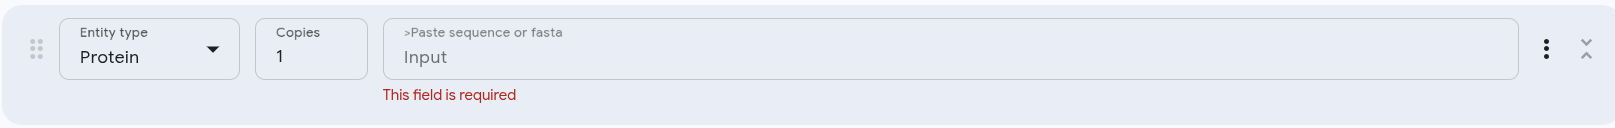
\includegraphics[width=0.95\textwidth]{../figures/af3_etapes/1_champ_vide.png}
  \caption{Étape 4 : la ligne d'entité vide, avant de coller la séquence.}
  \label{fig:af3_champ_vide}
\end{figure}

\begin{figure}[H]
\begin{enumerate}
  \setcounter{enumi}{4}
  \item Coller la séquence. Le serveur l'affiche découpée par blocs de 10, avec la numérotation au-dessus.
\end{enumerate}
  \centering
  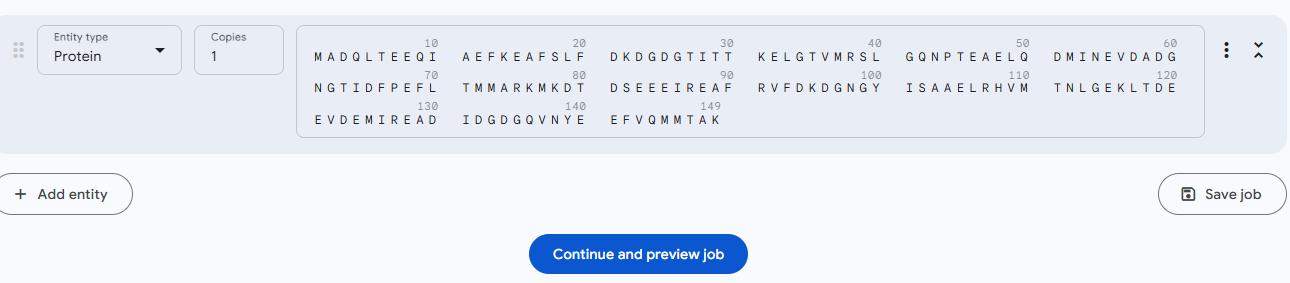
\includegraphics[width=0.95\textwidth]{../figures/af3_etapes/2_sequence_collee.png}
  \caption{Étape 5 : la séquence de l'ubiquitine collée (76 résidus), prête à être soumise.}
  \label{fig:af3_sequence}
\end{figure}

\begin{figure}[H]
\begin{enumerate}
  \setcounter{enumi}{5}
  \item Cliquer sur le bouton bleu \og Continue and preview job \fg{}. Une fenêtre récapitulative s'ouvre (figure~\ref{fig:af3_preview}) :
  \begin{itemize}
    \item \og Job name \fg{} : le serveur propose un nom (date et heure) ; le remplacer par \texttt{ubiquitine} pour retrouver la tâche facilement ;
    \item \og Seed \fg{} : laisser l'interrupteur désactivé (\og Seed: Auto \fg{}), le serveur tire alors une graine au hasard ;
    \item vérifier le tableau : \emph{Protein}, 1 copie, \og (length 76) \fg{}.
  \end{itemize}
  \item Cliquer sur \og Confirm and submit job \fg{}. Le compteur \og Remaining jobs \fg{} diminue de 1.
\end{enumerate}
  \centering
  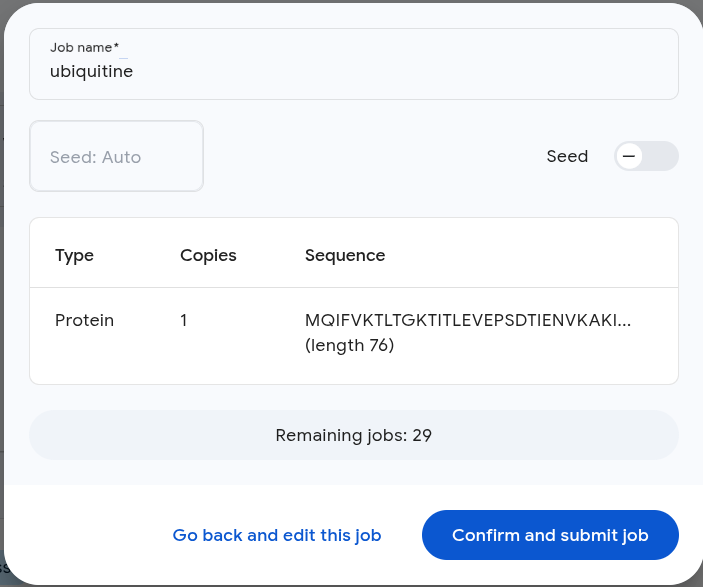
\includegraphics[width=0.55\textwidth]{../figures/af3_etapes/3_previsualisation.png}
  \caption{Étapes 6 et 7 : la fenêtre de prévisualisation avant l'envoi.}
  \label{fig:af3_preview}
\end{figure}

\begin{figure}[H]
\begin{enumerate}
  \setcounter{enumi}{7}
  \item Dans l'historique, sous le formulaire, attendre la fin du calcul (figure~\ref{fig:af3_historique}), puis cliquer sur le nom de la tâche.
\end{enumerate}
  \centering
  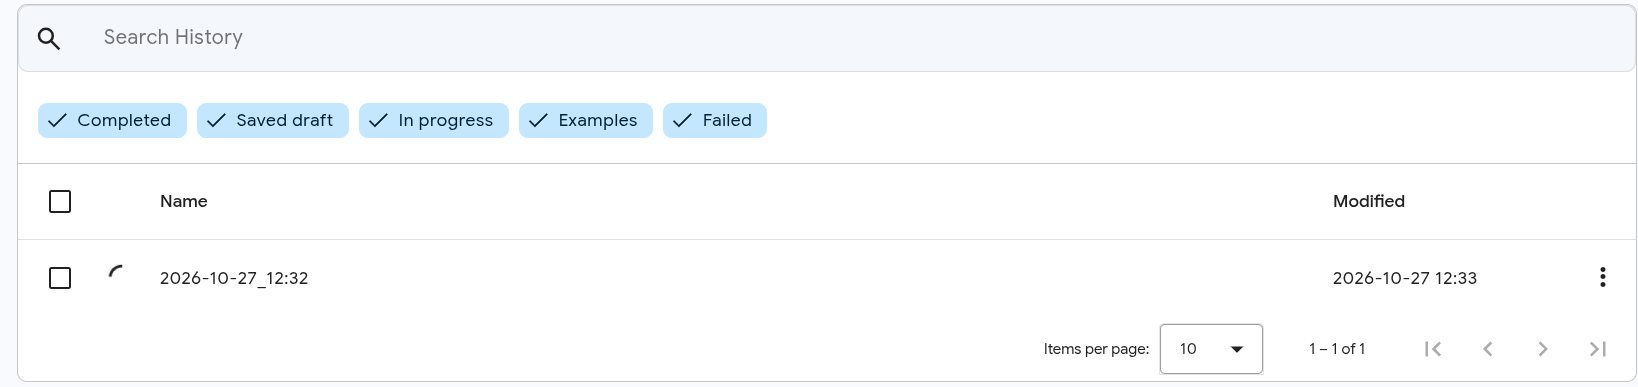
\includegraphics[width=0.95\textwidth]{../figures/af3_etapes/4_historique.png}
  \caption{Étape 8 : la tâche dans l'historique, en cours de calcul (icône de chargement à gauche du nom).}
  \label{fig:af3_historique}
\end{figure}

% À AJOUTER : capture d'écran du résultat AlphaFold Server, enregistrée sous figures/af3_ubiquitine.png
\begin{figure}[H]
\begin{enumerate}
  \setcounter{enumi}{8}
  \item Lire le résultat : la légende des couleurs pLDDT et les scores (\og ipTM = - \fg{}, \og pTM = 0.86 \fg{}) en haut, la structure 3D colorée par pLDDT à gauche et la matrice PAE à droite (figure~\ref{fig:af3_ubiquitine}).
\end{enumerate}
  \centering
  \IfFileExists{../figures/af3_ubiquitine.png}{%
    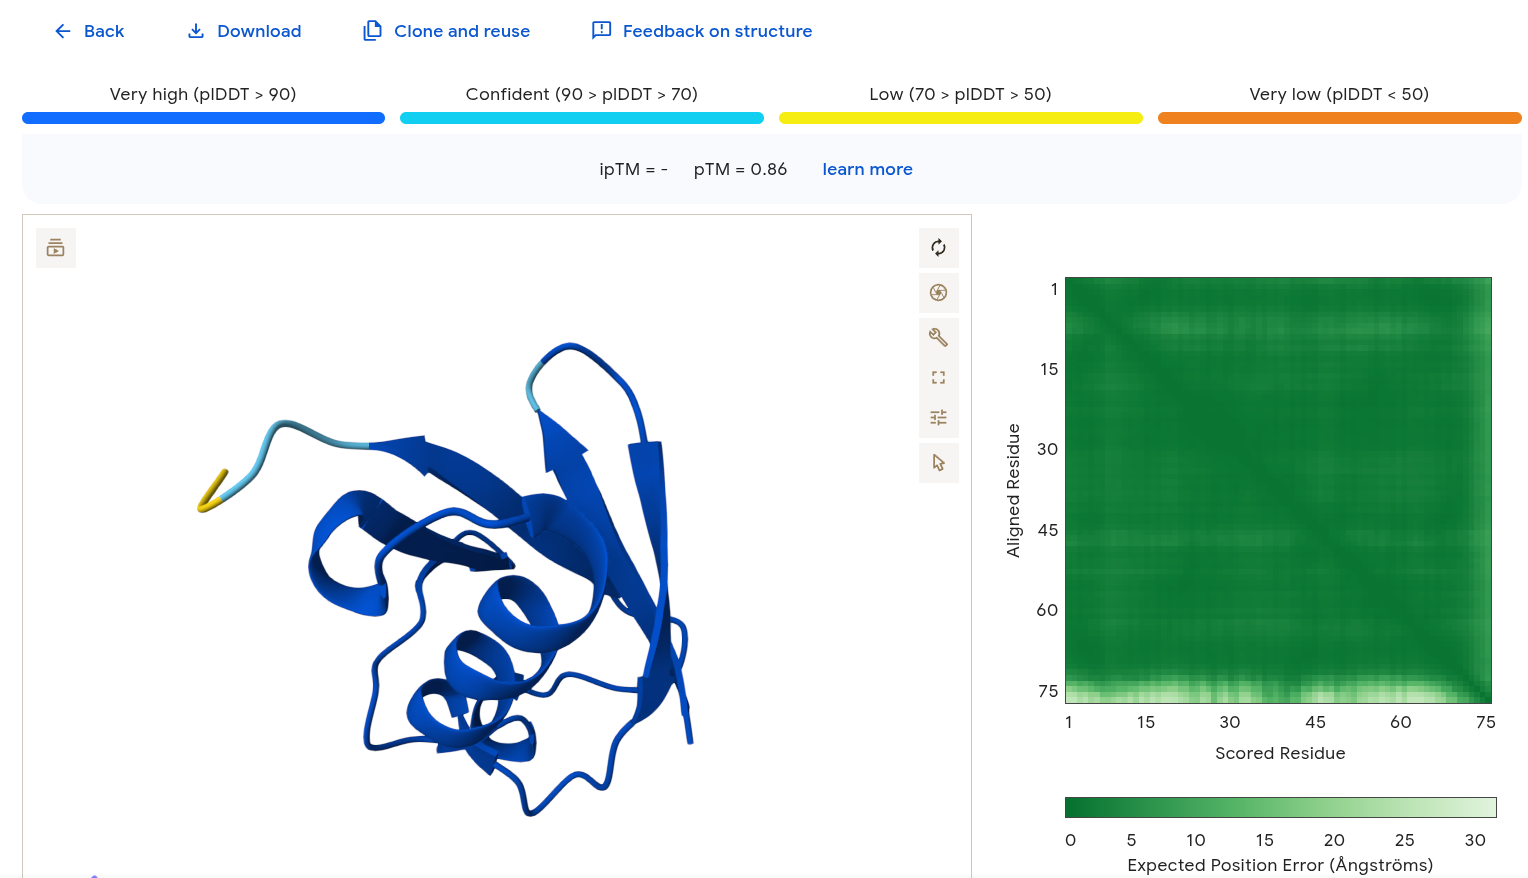
\includegraphics[width=0.95\textwidth]{../figures/af3_ubiquitine.png}%
  }{%
    \fbox{\parbox[c][4cm][c]{0.9\textwidth}{\centering Capture d'écran AlphaFold Server à ajouter\\(\texttt{figures/af3\_ubiquitine.png})}}%
  }
  \caption{Résultat d'AlphaFold3 (AlphaFold Server) pour l'ubiquitine : structure colorée par pLDDT (à gauche), matrice PAE (à droite) ; pTM = 0,86.}
  \label{fig:af3_ubiquitine}
\end{figure}

\paragraph{La forme.} La structure (figure~\ref{fig:af3_ubiquitine}) montre un \textbf{feuillet $\beta$} qui s'enroule autour d'une \textbf{hélice $\alpha$}. C'est le repliement \og $\beta$-grasp \fg{}, caractéristique de l'ubiquitine : compact et très stable.

\paragraph{Le pLDDT.} La légende d'AlphaFold Server reprend les classes de confiance d'AlphaFold2 : bleu foncé ($>$ 90), bleu clair (70--90), jaune (50--70) et orange ($<$ 50). L'ubiquitine est presque entièrement bleu foncé ; seule la queue C-terminale passe au bleu clair puis au jaune. Ce résultat est cohérent avec la biologie : cette queue flexible se termine par la glycine~76, qui se lie de façon covalente aux protéines cibles lors de l'ubiquitination.

\paragraph{La PAE.} La matrice est vert foncé presque partout : la protéine forme un seul bloc rigide, dont les positions relatives sont fiables. Seule une bande plus claire apparaît pour les résidus 72 à 76 : la position de la queue par rapport au reste de la protéine est incertaine. Sur une protéine à plusieurs domaines, on verrait au contraire plusieurs carrés foncés séparés par des zones claires, comme pour la calmoduline (figure~\ref{fig:pae}).

\paragraph{pTM et ipTM.} Le pTM vaut \textbf{0,86}, bien au-dessus du seuil de 0,5 au-delà duquel le repliement global est considéré comme correct. L'ipTM n'est pas défini ici (le serveur affiche \og ipTM = - \fg{}), puisqu'il n'y a qu'une seule chaîne. Il devient le score central dès que l'on ajoute une entité (seconde protéine, ADN, ligand). Il faut aussi savoir que le score TM est très sévère pour les petites structures : sous une vingtaine de jetons, le pTM est presque nul, et il vaut mieux se fier au pLDDT et à la PAE.

% PROLONGEMENT À FAIRE : soumettre la calmoduline (P0DP23) avec 4 ions Ca2+ sur AlphaFold Server
% et comparer le pLDDT, la PAE et l'orientation des lobes à la prédiction AlphaFold2 de la section sec:test.

%====================================================================
\section{Limites d'AlphaFold3}
%====================================================================

AlphaFold3 dépasse AlphaFold2, mais il ne règle pas tout.
\begin{itemize}
  \item \textbf{Des hallucinations.} Un modèle de diffusion produit toujours une structure, même là où il n'y en a pas. Dans les régions désordonnées, AlphaFold3 peut dessiner une hélice ou un repliement bien ordonné qui n'existe pas en réalité. Pour limiter ce défaut, ses auteurs l'ont entraîné aussi sur des prédictions d'AlphaFold-Multimer, où ces régions apparaissent sous forme de longues boucles étirées~\cite{abramson2024}. Il faut donc toujours lire le pLDDT avant d'interpréter une région.
  \item \textbf{Une structure statique.} Comme AlphaFold2, AlphaFold3 prédit un état stable. Il ne donne ni la dynamique, ni les changements de conformation, ni les affinités de liaison. Il ne remplace ni l'expérience, ni la dynamique moléculaire.
  \item \textbf{Des chimies nouvelles mal prédites.} La précision chute quand un ligand s'éloigne chimiquement de ceux vus à l'entraînement. Les complexes anticorps--antigène restent difficiles, malgré les progrès.
  \item \textbf{Un accès moins ouvert.} À sa sortie, ni le code ni les poids n'étaient publiés. Depuis fin 2024, le code est disponible, mais les poids sont accordés sur demande, pour un usage académique non commercial, et ne peuvent pas être redistribués~\cite{alphafold3_github}. AlphaFold2, lui, reste entièrement libre.
\end{itemize}

%====================================================================
\section{Et après ? Vers un \og AlphaFold~4 \fg{}}
%====================================================================

\paragraph{Pas d'AlphaFold~4 officiel.} À la date de ce rapport, Google DeepMind n'a publié aucun modèle nommé AlphaFold~4. L'expression circule pourtant depuis février 2026, à propos d'un modèle développé par \textbf{Isomorphic Labs}, la filiale de DeepMind consacrée à la découverte de médicaments.

\paragraph{IsoDDE, le successeur de fait.} Le 10 février 2026, Isomorphic Labs a présenté son \emph{Drug Design Engine} (\textbf{IsoDDE}) dans un rapport technique~\cite{isodde2026}. IsoDDE reprend les capacités de prédiction de structure d'AlphaFold3 et les complète par des modules dédiés à l'affinité de liaison, à la détection de poches et aux anticorps. Le biologiste computationnel Mohammed AlQuraishi (Columbia University) le décrit comme \og une avancée majeure, à l'échelle d'un AlphaFold~4 \fg{}~\cite{callaway2026}.

\paragraph{Pourquoi il serait meilleur qu'AlphaFold3.} Les gains annoncés visent précisément les limites d'AlphaFold3 décrites à la section précédente~\cite{isodde2026,callaway2026} :
\begin{itemize}
  \item \textbf{Des chimies nouvelles.} Sur le banc d'essai Runs N' Poses, pour les complexes protéine--ligand les plus éloignés des données d'entraînement (0 à 20~\% de similarité), IsoDDE fait plus de deux fois mieux qu'AlphaFold3. Il capte aussi l'ajustement induit, c'est-à-dire la déformation de la protéine au contact du ligand.
  \item \textbf{Les anticorps.} Sur 334 complexes anticorps--antigène peu similaires à l'entraînement, il obtient 2,3 fois plus de prédictions de haute qualité qu'AlphaFold3.
  \item \textbf{L'affinité de liaison.} AlphaFold3 donne une pose, pas une force de liaison. IsoDDE prédit l'affinité, avec une précision annoncée proche des calculs physiques de référence (perturbation d'énergie libre, FEP), sans structure cristallographique de départ et pour un coût bien moindre.
  \item \textbf{Les poches cachées.} À partir de la seule séquence, il a retrouvé des sites de liaison connus et nouveaux sur le céréblon, dont des poches \og cryptiques \fg{} qui n'apparaissent qu'en présence d'un ligand.
\end{itemize}
Autrement dit, AlphaFold3 répond à la question \og comment ce complexe est-il assemblé ? \fg{}. IsoDDE vise la question suivante du pharmacologue : \og cette molécule va-t-elle se fixer, où, et avec quelle force ? \fg{}.

\paragraph{Un progrès qu'on ne peut pas vérifier.} Contrairement à AlphaFold2 et AlphaFold3, IsoDDE est \textbf{propriétaire} : ni code, ni poids, ni serveur public, et le rapport ne décrit presque pas la méthode. Il est donc impossible de reproduire ces résultats, ni de savoir s'ils viennent d'innovations dans l'algorithme ou de données privées issues des partenariats industriels~\cite{callaway2026}. Ces chiffres sont des annonces de l'entreprise, pas des résultats évalués de façon indépendante. Il faut aussi noter la nature des sources : l'expression \og AlphaFold~4 \fg{} vient d'un article d'actualité de \emph{Nature} (rubrique \emph{News})~\cite{callaway2026}, qui rapporte l'avis de chercheurs, et non d'une publication scientifique évaluée par des pairs ; IsoDDE n'est lui-même décrit que dans un rapport technique de l'entreprise~\cite{isodde2026}.

\paragraph{Ce qui s'est passé depuis.} Huit mois après l'annonce d'IsoDDE, aucun modèle nommé AlphaFold~4 n'a été publié, ni par Google DeepMind, ni par Isomorphic Labs. Les nouvelles de 2026 vont plutôt dans le sens d'une fermeture :
\begin{itemize}
  \item \textbf{Mars--mai 2026} : seule avancée publique, AlphaFold DB s'ouvre aux complexes. EMBL-EBI, Google DeepMind, NVIDIA et l'Université nationale de Séoul y ont ajouté 1,7 million d'homodimères et près de 80\,000 hétérodimères prédits avec une confiance élevée, pour 20 espèces très étudiées et les pathogènes prioritaires de l'OMS~\cite{ebi_complexes2026}. Il s'agit de nouvelles prédictions, pas d'un nouveau modèle.
  \item \textbf{Mai 2026} : Isomorphic Labs lève 2,1 milliards de dollars (série~B menée par Thrive Capital, avec Alphabet et GV) pour développer IsoDDE et ses propres médicaments. L'annonce ne mentionne aucune ouverture du modèle~\cite{eurobiotech2026}.
  \item \textbf{Juillet 2026} : Google DeepMind dissout l'équipe dédiée à AlphaFold. Ses chercheurs sont réaffectés à des projets autour de Gemini, à d'autres recherches scientifiques ou à Isomorphic Labs, et John Jumper, colauréat du prix Nobel de chimie 2024 pour AlphaFold, quitte l'entreprise~\cite{engadget2026,gigazine2026}. AlphaFold DB, AlphaFold Server et AlphaFold3 restent toutefois disponibles.
\end{itemize}
Un AlphaFold~4 public, dans la lignée des versions précédentes, semble donc peu probable à court terme.

On retrouve ainsi, en plus marqué, la tendance déjà visible avec AlphaFold3 : à chaque génération, le modèle devient plus puissant, mais moins ouvert. AlphaFold2 était entièrement libre, AlphaFold3 l'est partiellement, et son successeur de fait est réservé à un usage interne. Pour la recherche publique, les alternatives ouvertes, comme Boltz-2, prennent le relais.

%====================================================================
\section{Retour d'expérience}
%====================================================================

\paragraph{Ce qui a fonctionné.} AlphaFold Server a rendu AlphaFold3 utilisable sans aucune installation ni GPU : une prédiction de l'ubiquitine se lance en quelques clics. Côté AlphaFold2, l'image Docker de ColabFold a fonctionné du premier coup sur une machine sans GPU, et toute la chaîne tient en deux commandes (\texttt{predict.sh} puis \texttt{analyse.py}).

\paragraph{Ce qui a posé problème.} Le temps de calcul d'AlphaFold2 sur CPU (1~h~57 pour 149 résidus) est prohibitif au-delà de quelques centaines de résidus. Pour AlphaFold3, l'obstacle n'est plus technique mais d'accès : sans GPU de 40 à 80~Go, seul le serveur est utilisable, avec son quota, sans API et avec une liste de ligands limitée.

\paragraph{Recommandations.}
\begin{itemize}
  \item Pour une protéine seule, AlphaFold2 (ColabFold) reste suffisant, libre et scriptable.
  \item Dès que la question porte sur une interaction (ADN, ARN, ligand, ion, autre protéine), utiliser AlphaFold3 via AlphaFold Server.
  \item Toujours lire le pLDDT \emph{et} la PAE avant d'interpréter la structure ; pour un complexe, regarder d'abord l'ipTM.
  \item Garder une trace des paramètres : graines, entités soumises, scores de confiance.
\end{itemize}
